\providecommand{\pdfxopts}{a-1b,cyrxmp}
\providecommand{\thisyear}{2021}
\immediate\write18{rm \jobname.xmpdata}%  uncomment for Unix-based systems
\begin{filecontents*}{\jobname.xmpdata}
	\Title{Лабораторные работы «Цифровая и микропроцессорная техника в управлении» с использованием «MexBIOS Development Studio 6.21»\textemdash\thisyear}
\Author{Артем Николаевич Прокшин, Александр Вячеславович Домнин, Варвара Дмитриевна Лиховская}
\Creator{pdfTeX + pdfx.sty with options \pdfxopts }
\Subject{Создание лабораторных работ по дисциплине «Цифровая и микропроцессорная техника в управлении» с использованием российского программного обеспечения
	«MexBIOS Development Studio 6.21»}
\Keywords{ковариантныые и контравариантрные координаты, MexBIOS Development Studio, электричесие машины}
\CoverDisplayDate{март \thisyear}
\CoverDate{2021-04-22}
\Copyrighted{True}
\Copyright{Public Domain}
\CopyrightURL{http://github.com/trot-t}
\Creator{pdfTeX + pdfx.sty with options \pdfxopts }
\end{filecontents*}

\documentclass[14pt]{beamer}

\pdfcompresslevel=9

\usepackage[\pdfxopts]{pdfx}[2016/03/09]
\PassOptionsToPackage{obeyspaces}{url}
\let\tldocrussian=1  % for live4ht.cfg

\usepackage[T2A]{fontenc}
\usepackage[utf8]{inputenc}
\usepackage[english,russian]{babel}
\usepackage{booktabs}
\usepackage{tikz}
\usepackage[european,cuteinductors,smartlabels]{circuitikz}
\usetikzlibrary{arrows.meta, shadows}

\usepackage{amssymb,amsfonts,amsmath,mathtext}
\usepackage{amssymb}
\usepackage{cite,enumerate,float,indentfirst}
\usepackage{cancel}
\usepackage{csquotes}
\newcommand{\quotes}[1]{``#1''}
\usetikzlibrary{calc}

\usepackage{advdate}

%\usepackage{pgfplots}
%\usepackage[left=1cm,right=1cm, top=1cm,bottom=1cm,bindingoffset=0cm]{geometry}

% Beamer — верстаем презентации  https://habrahabr.ru/post/145523/ 
\graphicspath{{images/}}

\usetheme{Pittsburgh}
\usecolortheme{whale}

\setbeamercolor{footline}{fg=blue}
\setbeamertemplate{footline}{
\leavevmode%
\hbox{%
\begin{beamercolorbox}[wd=.333333\paperwidth,ht=2.25ex,dp=1ex,center]{}%
Прокшин А.Н. и др.
\end{beamercolorbox}%
\begin{beamercolorbox}[wd=.333333\paperwidth,ht=2.25ex,dp=1ex,center]{}%
Санкт-Петербург, 2021
\end{beamercolorbox}%
\begin{beamercolorbox}[wd=.333333\paperwidth,ht=2.25ex,dp=1ex,right]{}%
Стр. \insertframenumber{} из \inserttotalframenumber \hspace*{2ex}
\end{beamercolorbox}}%
\vskip0pt%
}

\newcommand{\itemi}{\item[\checkmark]}

	\usefonttheme[onlymath]{serif} % в формулах использовать текст с засечками
\begin{document}
\title{\small{ Создание лабораторных работ по дисциплине \enquote{Цифровая и микропроцессорная техника в управлении} с использованием российского программного обеспечения
\enquote{MexBIOS Development Studio 6.21}}}
\author{\small{%
\emph{авторы:}~Александр Вячеславович Домнин, гр.8871\\%
\emph{}~Варвара Дмитриевна Лиховская, гр.8871\\
\emph{}~Прокшин Артем Николаевич}}



\institute{Санкт-Петербургский государственный электротехнический университет «ЛЭТИ» им. В.И. Ульянова (Ленина)}
\vspace{30pt}%

\vspace{60pt}%

\AdvanceDate[-4] % печатаю в субботу а нужна пятница
%\date{\small{Санкт-Петербург, 2021}}

\AtBeginSection{
	\begin{frame}
		\frametitle{Содержание}
		\tableofcontents[currentsection]
	\end{frame}
}

\begin{frame}
\titlepage	
\end{frame}

%\begin{frame}
%        \frametitle{Содержание}
%        \tableofcontents[currentsection] 
%\end{frame}
\begin{frame}
\frametitle{\small Цели, к которым стремились при реализации курса} 
\begin{itemize}
	\item упрощение системы управления с использованием ковариантных (измеряемых) и контравариантных (неизмеряемых) координат;
%\item использование дипломных проектов студентов; % предыдущих выпусков;
\item создание мобильных лабораторных стендов; % по тематике кафедры с перспективой на использование российских разработок;
\item использование российского программного обеспечения;
\item использование российских микроконтроллеров в части задач 
%\item оформление УМКД;
%\item ... будет сформулирована в результатах.
\end{itemize}
\end{frame}


\begin{frame}
\frametitle{\smallпрограммы -- бесплатно}
\begin{itemize}
	\item MexBIOS Development Studio 6.21 \cite{MexBios};
	\item MViewer \url{http://mviewer.ru} 
	\item Vector IDE
\end{itemize}
\end{frame}


\begin{frame}
\frametitle{\smallоборудование -- дешево} 
\begin{figure}
\begin{center}
\begin{minipage}[h]{0.5\linewidth}
\center{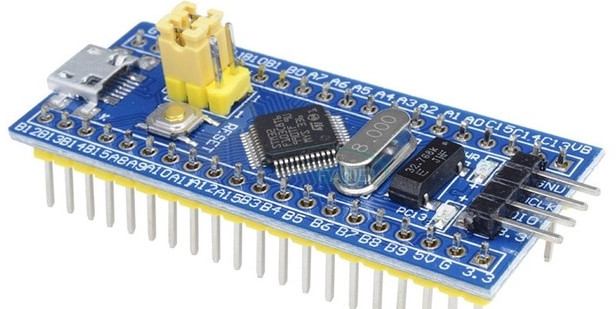
\includegraphics[width=1\linewidth]{stm32f103c8t6.jpg}}  \\
\end{minipage}
\end{center}
\end{figure} 
\begin{tabular}{ll}
микроконтроллер		&150 руб.\\
аппаратный программатор	&200-300 руб.\\
USB ком-порт	&150-200 руб.\\
светодиод,резистор,провода&100 руб.\\
\end{tabular}
\end{frame}


\begin{frame}
\frametitle{\smallоборудование -- дешево}
\begin{figure}
\begin{center}
\begin{minipage}[h]{0.5\linewidth}
\center{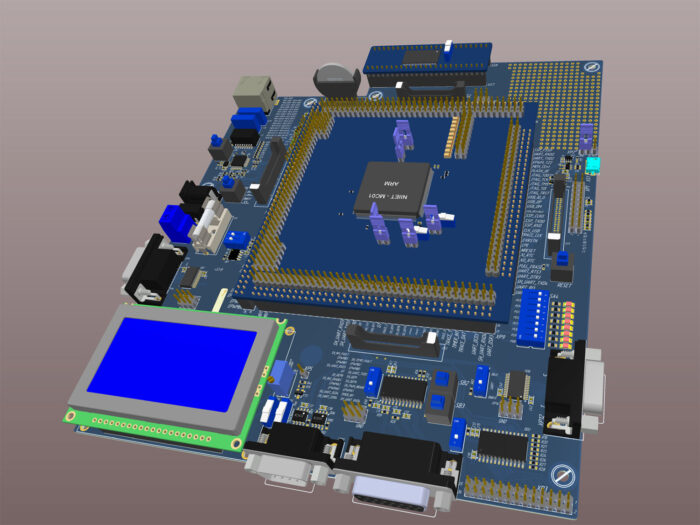
\includegraphics[width=1\linewidth]{2-3-700x525.jpg}}  \\
\end{minipage}
\end{center}
\end{figure}
\begin{tabular}{ll}
микроконтроллер К1921ВК01Т        &\\
макетная плата &\\
CAN-переходник Marathon &\\
\end{tabular}
\end{frame}



\begin{frame}
\frametitle{\small инвертор напряжения, принятые допущения}
	\hspace{-1cm}
\begin{figure}[!ht]
%\begin{figure}[!ht]
\hspace{-1cm}
\begin{circuitikz}[scale=0.82]
\ctikzset{bipoles/length=1.0cm}

\draw(1.25,2.65)node[nigbt,bodydiode](npn1){};% 1 ряд 
\draw (1.25,.55) node[nigbt,bodydiode](npn4){};%1ряд
\draw (npn1.S) -- (npn4.D);

% найдем положение плюсовой шины
\path let \p1 = (npn1.D) in node(plus)  at (0,\y1) {};
\draw (0,0) to[C] (plus);

\draw(2.75,2.65)node[nigbt,bodydiode](npn3){};% 2 ряд 
\draw (2.75,.55) node[nigbt,bodydiode](npn6){};% 2ряд
\draw (npn3.S) -- (npn6.D);

\draw (4.25,2.65)node[nigbt,bodydiode](npn5){};;%последний ряд 
\draw (4.25,.55) node[nigbt,bodydiode](npn2){};%последний ряд
\draw (npn5.S) -- (npn2.D);

\draw (plus.center) --(npn1.D) node[above]{1} -- (npn3.D) node[above]{3} -- (npn5.D) node[above]{5}; % плюсовая шина
\draw (0,0) |- (npn4.S) node[below]{4} -- (npn6.S) node[below]{6} -- (npn2.S) node[below]{2}; % минусовая шина

\ctikzset{iloop /.style={width=2.0}}

\draw ($(npn5.S)!1.0!(npn2.D)$)   node[left]{\scriptsize$C$} to[short,*-] ++ (0.5,0) to[iloop, name=Ic, mirror] ++(0.5,0) to[L,american inductor,-] ++ (1.5,0)  node(C) {};
\draw ($(npn3.S)!0.5!(npn6.D)$) node[left]{\scriptsize$B$} to[short,*-] ($(npn5.S)!0.5!(npn2.D)$) -- ++ (1.0,0) to[L,american inductor,-] ++ (1.5,0);  % катуха В 
\draw ($(npn1.S)!0.0!(npn4.D)$) node[left]{\scriptsize$A$}  to[iloop, name=Ia, mirror,*-] ++(1.5,0) to[short] ($(npn5.S)!0.0!(npn2.D)$) -- ++ (1.0,0) to[L,american inductor,l={\small },-] ++ (1.5,0) node(A) {};

\draw (A.center)--(C.center) (A.center) --++(0,1.5) (C.center) --++ (0,-1.5);

\draw (A.center) ++(0.1,0.8) --++ (-0.2,0.2);
\draw (A.center) ++(0.1,0.9) --++ (-0.2,0.2);
\draw (A.center) ++(0.1,1.0) --++ (-0.2,0.2);

\draw (Ia) --++ (0,-2.5) node[below] {\small $i_A$}; 
\draw (Ic) --++ (0,-2) node[below] {\small $i_C$}; 
\end{circuitikz}
\hspace{-0.1cm}
\begin{circuitikz}[scale=0.83]
\newcommand{\D}{2.4}
\newcommand{\I}{1.85}
\draw[thin] (0,0) --({\D*cos(0)},{\D*sin(0)})   node(A) {} node[right] {\tiny 100};
\draw[thin] (0,0) --({\D*cos(60)},{\D*sin(60)}) node(W) {} node[above right] {\tiny 110};
\draw[thin] (0,0) --({\D*cos(120)},{\D*sin(120)}) node(B) {} node[above left] {\tiny 010};
\draw[thin] (0,0) --({\D*cos(180)},{\D*sin(180)}) node(U) {} node[left] {\tiny 011 };
\draw[thin] (0,0) --({\D*cos(240)},{\D*sin(240)}) node(C) {} node[below left] {\tiny 001 };
\draw[thin] (0,0) --({\D*cos(300)},{\D*sin(300)}) node(V) {} node[below right] {\tiny 101};
\draw[thin] (A.center) -- (W.center) -- (B.center) -- (U.center) -- (C.center) -- (V.center) -- (A.center);
\draw[very thin,red,dashed] (0,0) circle ({\I});
\draw[fill, white] ({\I*cos(25)},{\I*sin(25)})  rectangle  ({\I*cos(25)+0.5},{\I*sin(25)+0.5});
\draw[->,>=latex,thick,red] (0,0) -- ({\I*cos(25)},{\I*sin(25)}) node[above right] {$\vec{u}$};
\end{circuitikz}
% \caption{схема инвертора напряжения ведомого сетью и изображающий вектор напряжения инвертора}
% \label{invertor_with_grid}
%\end{figure}

%        \caption{схема инвертора напряжения ведомого сетью и изображающий вектор напряжения инвертора}
%        \label{invertor_with_grid}
\end{figure}
\end{frame}

%\section{проекции пространственного вектора}
\frame{\frametitle{\small проекции пространственного вектора тока в выбранной фазе}
\vspace{-1cm}
\begin{table}%
        \flushleft
\begin{tabular}{@{}p{4.5cm}p{9cm}@{}}%
\parbox[t]{4.5cm}{
\begin{circuitikz}
        \draw (0,0) to[sV] (0,2.5) to[R,l={$R$}] (2,2.5) to[short, i>=$P\!\sim\!I^2 R$] (4,2.5) -- (4,0) -- (0,0);
\end{circuitikz}
}
        &
\only<2,3>{
%\parbox[t]{6cm}{
        \begin{circuitikz}
        \newcommand{\D}{2.5}
        \draw[thin,->,>=latex] (-2.5,0) -- (2.5,0);
        \draw[thin,->,>=latex] (0,-2) -- (0,2);
		\draw[thick,->,>=latex,blue] (0,0) -- ({\D*cos(30)}, {\D*sin(30)}) node[above right] {$\vec{i}$};
        \draw[thin,dashed] ({\D*cos(30)}, {\D*sin(30)}) -- ({\D*cos(30)}, 0) node[below] {$I\cos\omega t$};
        \end{circuitikz}
%}
        } \\
\end{tabular}
\end{table}
\only<3>{
\vspace{1cm}
Измеряемая величина -- \\перпендикулярная проекция вектора $\vec{i}$ на ось фазы A
}
} % frame


\begin{frame}
\frametitle{\small измеряемые координаты изображающего вектора}
$$
	\vec{i} = \frac{2}{3}\left(\vec{i}_{a_{\!\perp}} + \vec{i}_{b_{\!\perp}} + \vec{i}_{c_{\!\perp}}\right) 
$$
%
\begin{tabular}{cl}
\begin{minipage}[h]{0.3\linewidth}
\begin{tikzpicture}[scale=2]
\newcommand{\D}){8}
\draw[->, very thin,>=latex] (0,0) -- (1.00, 0.00);
\draw[->, very thin,>=latex] (0,0) -- ({cos(120)},{sin(120)});
\draw[->, very thin,>=latex] (0,0) -- ({cos(240)},{sin(240)});

\draw[yellow, very thick,->,>=latex] (0,0) -- (0.59,0);
\draw[green, very thick,->,>=latex] (0,0) -- (-0.20,0.35);
\draw[red, very thick,->,>=latex] (0,0) -- (0.50,0.86);
\draw[->,thick] (0,0) -- (0.59, 0.81) node[above right] {$\vec{i}$};
\end{tikzpicture} 
\end{minipage}
&
\begin{minipage}[h]{0.7\linewidth}
	{\small\begin{itemize}
\item измеряемые величины -- перпендикулярные координаты вектора \cite{Gorev},\cite{Sokolovsky}; 
%\item физическая величина -- всегда произведение  ко- и контра-вариантных координат;
%\item изображающий вектор симметричной системы есть $2/3 (I_a + I_b + I_c)$;
%\item рисунок -- есть результат 1й практической работы.
\end{itemize}
	}
\end{minipage}
\end{tabular}
\end{frame}


\begin{frame}
\frametitle{\small использование измерений в системе управления}
\begin{figure}
\begin{center}
%\begin{minipage}[h]{0.5\linewidth}
\center{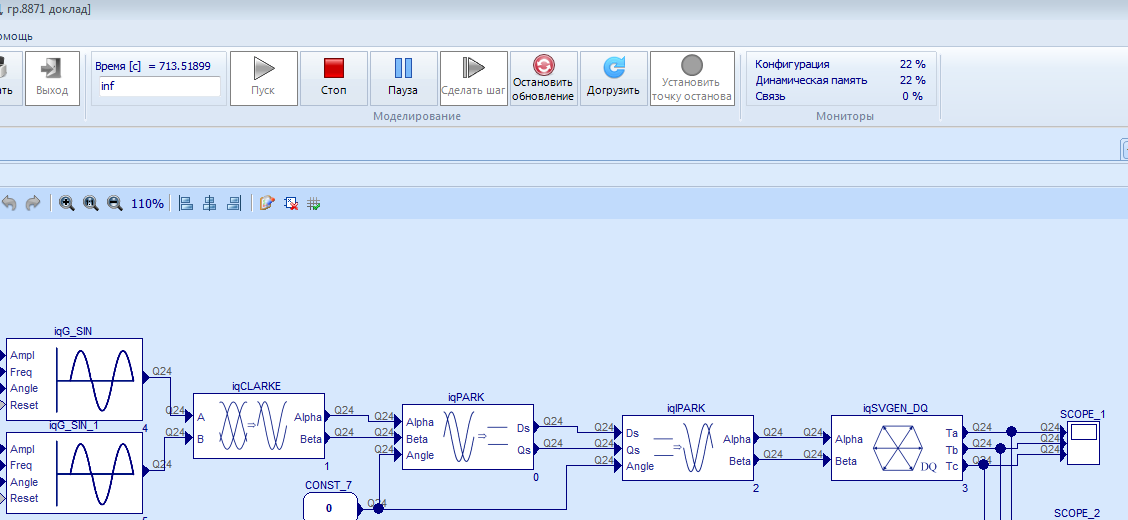
\includegraphics[width=1\linewidth]{classic.png}}  \\
%\end{minipage}
\end{center}
\end{figure}
	Часто используемая последовательность блоков 
	системы управления \cite{Gorev},\cite{Sokolovsky} 
	: преобразования Кларка, Парка-Горева, обратные преобразования Парка-Горева, Кларка (обратные связи опущены).
\end{frame}


\frame{\frametitle{\small длина вектора, ковариантные и контрaвариантные координаты}

\begin{columns}
\hspace{-1cm}
        \begin{column}{0.45\textwidth}

\begin{circuitikz}
        \newcommand{\I}{3.2}
        \newcommand{\teta}{120}
        \newcommand{\alfa}{25}

        \newcommand{\X}{\I*cos(\alfa)}
        \newcommand{\Y}{\I*sin(\alfa)}
        \newcommand{\Yaxe}{4}
        % ось
	\draw[very thin,->,>=latex] (0,0) -- (4,0) node[right] {\only<1>{\small $I_A$}};
	\draw[very thin, ->,>=latex] ({1*cos(-60)},{1*sin(-60)}) -- ({\Yaxe*cos(\teta)},{\Yaxe*sin(\teta)}) node[right] {\small $I_B$};

        \draw[->,>=latex] (0,0) -- ({\I*cos(\alfa)}, {\I*sin(\alfa)}) node[above right] {$\vec{i}$};
        % проекция на ось Х
        \draw[very thin, loosely dashed] ({\X},{\Y}) -- ({\X-\Y*cos(\teta)/sin(\teta)}, 0) node[below] {$i^A$};

        \draw[thin, dotted] ({\X},{\Y}) -- ({\X},0) node[below] {$i_A$};
        % проекция на ось Y

        \draw[very thin,loosely dashed] ({\X}, {\Y}) -- ( {\Y*cos(\teta)/sin(\teta)} ,{\Y}) node[left] {$i^B$};
        % перпендикуляр на ось Y
        \newcommand{\perpend}{\I*cos(\teta-\alfa)}
        \draw[thin,dotted] ({\X}, {\Y}) -- ({\perpend*cos(\teta)},{\perpend*sin(\teta)}) node[below left] {$i_B$};
\end{circuitikz}
		$$ \mid\! \vec{i}\!\mid^2 = i_A\cdot i^A + i_B\cdot i^B $$ 
        \end{column}
\begin{column}{0.55\textwidth}
        \only<2>{
\begin{circuitikz}
        \newcommand{\I}{3.2}
        \newcommand{\teta}{65}
        \newcommand{\alfa}{25}

        \newcommand{\X}{\I*cos(\alfa)}
        \newcommand{\Y}{\I*sin(\alfa)}
        \newcommand{\Yaxe}{4}
        % ось
	\draw[very thin,->,>=latex] (0,0) -- (4,0) node[above right] {\small{$X_1$}};
        \draw[very thin, ->,>=latex] (0,0) -- ({\Yaxe*cos(\teta)},{\Yaxe*sin(\teta)}) node[right] {\small{$X_2$}};

        % вектор
        \draw[->,>=latex] (0,0) -- ({\I*cos(\alfa)}, {\I*sin(\alfa)}) node[above right] {\small{$\mid\vec{x}\mid=1$}};
        % обозначение угла \alfa
        \draw[blue,thin,<->] (1,0) arc(0:{\alfa}:1) node[midway,right=-1.4mm] {\tiny{$\alpha$}};
        % параллельная проекция на ось X1
        \draw[very thin, loosely dashed] ({\X},{\Y}) -- ({\X-\Y*cos(\teta)/sin(\teta)}, 0) node[below] {\small{$x^1$}};
        % перпендикуляр на ось X1
        \draw[thin, dotted] ({\X},{\Y}) -- ({\X},0) node[below right] {\small{$x_1 = \cos\alpha$}};

        % проекция x^1 на вектор I
        \newcommand{\XX}{(\X-\Y*cos(\teta)/sin(\teta))*cos(\alfa) }
        \draw[thin, dotted] ({\X-\Y*cos(\teta)/sin(\teta)},0) -- ({\XX*cos(\alfa)}, {\XX*sin(\alfa)}) node[above] {\tiny{$x^1\!\!\cos\alpha$}};

        % обозначение угла \beta
        \draw[red,thin,<->] ({0.7*cos(\alfa)},{0.7*sin(\alfa)}) arc({\alfa}:{\teta}:0.7) node[midway,above right=-1.4mm] {\tiny{$\beta$}};
        % проекция на ось X2
        \draw[very thin,loosely dashed] ({\X}, {\Y}) -- ({\Y*cos(\teta)/sin(\teta)} ,{\Y}) node[left] {\small{$x^2$}};
        % перпендикуляр на ось Y
        \newcommand{\perpend}{\I*cos(\teta-\alfa)}
        \draw[thin,dotted] ({\X}, {\Y}) -- ({\perpend*cos(\teta)},{\perpend*sin(\teta)}) node[above left] {\small{$\cos\beta\!=\!x_2$}};

        % проекция x^2 на вектор I
        \newcommand{\YY}{\I*sin(\alfa)/sin(\teta)*cos(\teta-\alfa)}
        \draw[thin, dotted] ({\Y*cos(\teta)/sin(\teta)} ,{\Y}) -- ({\YY*cos(\alfa)}, {\YY*sin(\alfa)}) node[right] {\tiny{$x^2\!\!\cos\beta$}};
\end{circuitikz}
        }
\end{column}
\end{columns}
\vspace{0.5cm}
физическая величина -- произведение  ко- и контра-вариантных координат
}

\frame{\frametitle{\smallосновной и сопряженный базис, разложение по базисам}
\begin{columns}
\begin{column}{0.45\textwidth}
\begin{circuitikz}
        \newcommand{\I}{3.5}

        \newcommand{\teta}{120}
        \newcommand{\alfa}{25}
        \newcommand{\sopr}{30}

        \newcommand{\X}{\I*cos(\alfa)}
        \newcommand{\Y}{\I*sin(\alfa)}
        \newcommand{\Xaxe}{3}
        \newcommand{\Yaxe}{3}
        \newcommand{\Xsopr}{\Xaxe*2/sqrt(3)}
        \newcommand{\Ysopr}{\Yaxe*2/sqrt(3)}

        % основной базис
        \draw[very thin,->,>=latex] (0,0) -- (\Xaxe,0) node[below] {$\vec{g}_1$};
        \draw[very thin, ->,>=latex] (0,0) -- ({\Yaxe*cos(\teta)},{\Yaxe*sin(\teta)}) node[above right] {$\vec{g}_2$};

        %
        \draw[very thin,->,>=latex] (0,0) -- ({\Xsopr*cos(\sopr)},{\Xsopr*sin(\sopr)}) node[above right] {$\vec{g}^1$};
        \draw[very thin,->,>=latex] (0,0) -- (0,{\Ysopr}) node[right] {$\vec{g}^2$};

        % сетка возрастания координаты x^2
        \newcommand{\dd}{0.4*2/sqrt(3)}
        \draw[very thin, red] ({\dd*cos(\teta)},{\dd*sin(\teta)}) -- (1.9,{\dd*sin(\teta)}) node[right] {\small{$x^2\!=\!const_1$}};
        \draw[very thin, red] ({2*\dd*cos(\teta)},{2*\dd*sin(\teta)}) -- (1.9,{2*\dd*sin(\teta)}) node[right] {\small{$x^2\!=\!const_2$}};
\end{circuitikz}

        \vspace{-0.5cm}
\small{
$$
\begin{array}{cc}
        \left(\vec{g^1} \cdot \vec{g}_1\right) \!=\! 1; &\left(\vec{g^1} \cdot \vec{g}_2\right) = 0; \\
        \left(\vec{g^2} \cdot \vec{g}_1\right) \!=\! 0; &\left(\vec{g^2} \cdot \vec{g}_2\right) = 1; \\
\end{array}
$$
$$
        \left(\vec{g^i} \cdot \vec{g}_j\right)  = \delta^i_j = \delta^{i~}_{~j}
$$
}
\end{column}
\begin{column}{0.55\textwidth}
        \only<2>{
        \small{
\noindentразложение вектора по базисy:
        \vspace{-0.3cm}
        $$
        \vec{x} = x^1\vec{g}_1 + x^2\vec{g}_2 = \sum\limits_{i=1}^2 x^i\vec{g}_i = x^i\vec{g}_i
        $$
        $$
        \vec{x} = x_1\vec{g^1} + x_2\vec{g^2} = x_i\vec{g^i}
        $$
        \vspace{0.8cm}

вычисление координат:
$$
(\vec{x} \cdot \vec{g^i} ) \!=\! x^i
$$
$$
(\vec{x} \cdot \vec{g}_i ) \!=\! x_i
$$
}
}
\end{column}
\end{columns}
}

\frame{\frametitle{\small как найти контрaвариантные координаты}

Формула для мощности в инверторе
$$
p = i_A \cdot u^A + i_B \cdot u^B
$$
Как найти контравариантые координаты?
\begin{itemize}
\item симметрия системы;
\item из системы управления -- при генерации $u$ пользуемся контравариантными координатами;
\item оси измерения линейных напряжений $u_{\scriptscriptstyle AB}$ и $u_{\scriptscriptstyle BC}$ сопряжены с осями измерений $i_{\scriptscriptstyle A}$ и $i_{\scriptscriptstyle (-C)}$ 
\end{itemize}
}

\frame{
\frametitle{\small контравариантные координаты -- симметрия системы}
\begin{circuitikz}
        \newcommand{\I}{3}

        \newcommand{\alfa}{40}
        \newcommand{\teta}{120}
        \newcommand{\tepa}{240}

        \newcommand{\Xaxe}{4.2}
        \newcommand{\Yaxe}{4.2}

        \draw[very thin, ->,>=latex] (0,0) -- ({\Xaxe},0) node[below right] {$A$};
        \draw[very thin, ->,>=latex] (0,0) -- ({\Xaxe*cos(\teta)},{\Xaxe*sin(\teta)}) node[right] {$B$};
        \draw[very thin] (0,0) -- ({\Xaxe*cos(60)},{\Xaxe*sin(60)});
        \draw[very thin, ->,>=latex] (0,0) -- ({\Yaxe*cos(\tepa)},{\Yaxe*sin(\tepa)}) node[right] {$C$};
        \draw[very thin] (0,0) -- ({\Xaxe*cos(-60)},{\Xaxe*sin(-60)});

        \draw[thick,red,->,>=latex] (0,0) -- ({\I*cos(\alfa)},{\I*sin(\alfa)});

	\draw[thin,dashed] ({\I*cos(\alfa)},{\I*sin(\alfa)}) -- ({\I*cos(\alfa)}, 0 ) node[below=-1mm] {\tiny{$i^{~~ab}_A$}} node[below=2.5mm] {\tiny{$i_A^{~~ac}$}} ;
	\draw[thin,dotted] ({\I*cos(\alfa)},{\I*sin(\alfa)}) -- ({\I*cos(\alfa) - \I*sin(\alfa)/tan(60)}, 0 ) node[below right=-1.5mm] {\tiny{$i^A_{~~ac}$}};;
	\draw[thin,dotted] ({\I*cos(\alfa)},{\I*sin(\alfa)}) -- ({\I*cos(\alfa) + \I*sin(\alfa)/tan(60)}, 0 ) node[below=-1mm] {\tiny{$i^A_{~~ab}$}};

        \draw[thin,dotted] ({\I*cos(\alfa)},{\I*sin(\alfa)}) -- ({\I*sin(\alfa)/tan(120)}, {\I*sin(\alfa)}) node[left] {\tiny{$i^B_{~~ab}$}};
        \draw ({\I*sin(\alfa)/tan(60)}, {\I*sin(\alfa)}) node[below left=-1.5mm] {\tiny{$x_{~ac}^C~~$}};
        \newcommand{\Oo}{(\teta-\alfa)}
        \draw[thin,dashed] ({\I*cos(\alfa)},{\I*sin(\alfa)}) -- ({\I*cos(\Oo)*cos(\teta)},{\I*cos(\Oo)*sin(\teta)}) node[left=-1mm] {\tiny{$x^{~~ab}_B\!=\!x^{~~bc}_B$}};
        \newcommand{\Ooo}{(60-\alfa)}
        \newcommand{\DD}{\I*cos(\Ooo)}
        \draw[thin,dashed] ({\I*cos(\alfa)},{\I*sin(\alfa)}) -- ({\DD*cos(60)},{\DD*sin(60)}) node[left=-0mm] {\tiny{$x^{~~ac}_C\!=\!x^{~~bc}_C$}};
        \newcommand{\DDD}{(\I*cos(\alfa) + \I*sin(\alfa)/tan(60))}
        \draw[thin,dotted] ({\I*cos(\alfa)},{\I*sin(\alfa)}) -- ({\DDD*cos(60)},{\DDD*sin(60)}) node[above left=-1.5mm] {\tiny{$x_{~~bc}^C$}};
        \newcommand{\DDDD}{(\I*cos(\alfa) - \I*sin(\alfa)/tan(60))}
        \draw[thin,dotted] ({\DDDD}, 0 ) -- ({\DDDD*cos(-60)},{\DDDD*sin(-60)}) node[below left=-1mm] {\tiny{$x_{~~bc}^B$}};
	\draw(3,-2) node[right] {$\vec{i} = \frac{2}{3}\left(i_{\scriptscriptstyle A} \vec{e}_{\scriptscriptstyle A} +
	i_{\scriptscriptstyle B} \vec{e}_{\scriptscriptstyle B} + i_{\scriptscriptstyle C} \vec{e}_{\scriptscriptstyle C}
	\right)$};
\end{circuitikz}
}

\begin{frame}
\frametitle{\small контравариантные координаты -- управление}
	\begin{tikzpicture}[scale=0.8]
\newcommand{\D}{8} % длина стороны треугольника
\newcommand{\vx}{5}
\newcommand{\vy}{2}
		\draw[thick] (0,0) node[below left] {$\small{\bf{(000)}\over{(111)}}$~~ {\large${\bf  m_1}$}} -- ({\D},0) node[below right] {{\large${\bf m_2~\scriptstyle{(100)}}$}} -- 
		({\D/2},{\D*sqrt(3)/2}) node[above=8] {{\large${\bf m_3~\scriptstyle{(110)}}$}} -- (0,0);
%       \draw[red,thick,->,>=stealth'] (0,0) -- ({\vx}, {\vy}) node(v) {};
%	\draw[thin] ({\vx + \vy/tan(60)},0) -- (\vx,\vy) -- ({(\vx + \vy/tan(60))/2}, {(\vx + \vy/tan(60))*sqrt(3)/2} ); % контравариантная на ось фазы C и на ось фазы А

	% сам вектор 
        \draw[red,very thick,->,>=latex] (0,0) -- ({\vx}, {\vy}) node(v) {};


\only<1>{
	\draw[thin] ({\vy/tan(60)} ,{\vy}) --  ({\vx}, {\vy}) -- ({\D - \vy/tan(60)},{\vy}); % node[midway, below right=-0.05cm] {$m_1$};	
	\draw[very thin] (0,-1.5) -- (0,-1.5); % только для того чтобы выровнять 1й рисунок как и на остальных страницах
}	
	
\only<2,3>{
	
	\draw[thin] ({\vx + \vy/tan(60)},0) -- (\vx,\vy) -- ({(\vx + \vy/tan(60))/2}, {(\vx + \vy/tan(60))*sqrt(3)/2} ); % контравариантная на ось фазы C и на ось фазы А
        % подписи внизу
        \draw[very thin] (0,-0.1) -- (0,-1.5);
        \draw ({\vx + \vy/tan(60)},-0.1) -- ({\vx + \vy/tan(60)},-0.8); \draw (\D,-0.1) -- (\D,-1.5);
        \draw[very thin,<->,>=latex] (0,-0.4) --  ({\vx + \vy/tan(60)}, -0.4) node[midway, below] {$m_2+m_3$};
        \draw[very thin,<->,>=latex]  ({\vx + \vy/tan(60)}, -0.4) -- (\D, -0.4) node[midway, below] {$m_1$};
}
\only<2>{	\draw[very thin] (0,0) -- ({\D*cos(30)*(sqrt(3)/2)},{\D*sin(30)*(sqrt(3)/2)});  % перпендикуляр
        \newcommand{\perpend}{0.3} % для перпендикуляра
		\draw ({\D*cos(30)*(sqrt(3)/2) + \perpend*cos(120)},{\D*sin(30)*(sqrt(3)/2) + \perpend*sin(120)}) --++ ({\perpend*cos(210)},{\perpend*sin(210)}) --++ ({\perpend*cos(300)},{\perpend*sin(300)});
	% конец вектора
	\draw ({\vx}, {\vy})  node[below=0.15cm] {\small$o^\prime$};	


	}
\only<3>{
	% конец вектор
	\draw ({\vx}, {\vy})  node[above=0.25cm] {$o^\prime$};
        \draw[thin] ({\vy/tan(60)} ,{\vy}) --  ({\vx}, {\vy}) -- ({\D - \vy/tan(60)},{\vy}) node[midway, below right=-0.05cm] {$m_1$};
        \draw[thin] ({\vx-\vy/tan(60)},0 ) -- (\vx,\vy); 
        \draw[thin] ({\D/2 + (\vx-\vy/tan(60))/2}, {\D*sqrt(3)/2 - (\vx-\vy/tan(60))*sqrt(3)/2}) -- (\vx,\vy) node[midway, above=0.25cm] {$m_1$}; % контравариантная на ось фазы B || [1-3]

        \draw[very thin]  ({\vx - \vy/tan(60)}, -1.0) -- ({\vx - \vy/tan(60)}, -1.5);
        \draw[very thin,<->,>=latex]  (0,-1.2) --  ({\vx - \vy/tan(60)}, -1.2) node[midway, below] {$m_2$};
        \draw[very thin,<->,>=latex] ({\vx - \vy/tan(60)}, -1.3) -- (\D, -1.3) node[midway, below] {$m_1+m_3$};
 
        % подписи справа
        \draw[very thin] ({\D + 0.1*sqrt(3)/2}, {0 + 0.1/2}) -- ({\D + 0.8*sqrt(3)/2}, {0 + 0.8/2});
        \draw[very thin] ({\D - \vy/tan(60) + 0.1*sqrt(3)/2} ,{\vy + 0.1/2}) -- ({\D - \vy/tan(60) + 0.8*sqrt(3)/2},{\vy + 0.8/2});
        \draw[very thin,<->,>=latex] ({\D + 0.5*sqrt(3)/2}, {0 + 0.5/2}) -- ({\D - \vy/tan(60) + 0.5*sqrt(3)/2} ,{\vy + 0.5/2}) node[midway, above right] {$m_3$};
        \draw[very thin] ({\D/2 + (\vx-\vy/tan(60))/2 + 0.1*sqrt(3)/2}, {\D*sqrt(3)/2 - (\vx-\vy/tan(60))*sqrt(3)/2 + 0.1/2}) --
                          ({\D/2 + (\vx-\vy/tan(60))/2 + 0.8*sqrt(3)/2}, {\D*sqrt(3)/2 - (\vx-\vy/tan(60))*sqrt(3)/2 + 0.8/2});
        \draw[very thin,<->,>=latex] ({\D - \vy/tan(60) + 0.65*sqrt(3)/2} ,{\vy + 0.65/2}) --
                                        ({\D/2 + (\vx-\vy/tan(60))/2 + 0.65*sqrt(3)/2}, {\D*sqrt(3)/2 - (\vx-\vy/tan(60))*sqrt(3)/2 + 0.65/2}) node[midway, above right] {$m_1$};
        \draw[very thin] ({\D/2 + 0.1*sqrt(3)/2},{\D*sqrt(3)/2 + 0.1/2}) -- ({\D/2 + 0.8*sqrt(3)/2},{\D*sqrt(3)/2 + 0.8/2});
        \draw[very thin,<->,>=latex] ({\D/2 + 0.55*sqrt(3)/2} ,{\D*sqrt(3)/2 + 0.55/2}) --
                                        ({\D/2 + (\vx-\vy/tan(60))/2 + 0.55*sqrt(3)/2}, {\D*sqrt(3)/2 - (\vx-\vy/tan(60))*sqrt(3)/2 + 0.55/2}) node[midway, above right] {$m_2$};
        %подписи слева
        \draw[very thin] ({0 - 0.1*sqrt(3)/2}, {0 + 0.1/2}) -- ({0 - 0.8*sqrt(3)/2}, {0 + 0.8/2});
        \draw[very thin] ({\vy/tan(60) - 0.1*sqrt(3)/2} ,{\vy + 0.1/2}) -- ({\vy/tan(60) - 1.1*sqrt(3)/2} ,{\vy + 1.1/2});
        \draw[very thin,<->,>=latex] ({0 - 0.75*sqrt(3)/2}, {0 + 0.75/2}) -- ({\vy/tan(60) - 0.75*sqrt(3)/2} ,{\vy + 0.75/2}) node[midway, above left] {$m_3$};
        \draw[very thin] ({(\vx + \vy/tan(60))/2 - 0.1*sqrt(3)/2}, {(\vx + \vy/tan(60))*sqrt(3)/2 + 0.1/2}) --
                         ({(\vx + \vy/tan(60))/2 - 1.1*sqrt(3)/2}, {(\vx + \vy/tan(60))*sqrt(3)/2 + 1.1/2});
        \draw[very thin,<->,>=latex] ({\vy/tan(60) - 0.9*sqrt(3)/2} ,{\vy + 0.9/2}) --
                                        ({(\vx + \vy/tan(60))/2 - 0.9*sqrt(3)/2}, {(\vx + \vy/tan(60))*sqrt(3)/2 + 0.9/2}) node[midway, above left] {$m_2$};
        \draw[very thin] ({\D/2 - 0.1*sqrt(3)/2},{\D*sqrt(3)/2 + 0.1/2}) --  ({\D/2 - 0.8*sqrt(3)/2},{\D*sqrt(3)/2 + 0.8/2});
        \draw[very thin,<->,>=latex]  ({(\vx + \vy/tan(60))/2 - 0.5*sqrt(3)/2}, {(\vx + \vy/tan(60))*sqrt(3)/2 + 0.5/2}) --
                                         ({\D/2 - 0.5*sqrt(3)/2},{\D*sqrt(3)/2 + 0.5/2}) node[midway, above left] {$m_1$}; 
}
%\only<4>{
%	% вспомогательная ось B
%        \draw[ultra thin] ({-0.7*cos(-60)},{-0.7*sin(-60)}) -- ({1.2*cos(-60)},{1.2*sin(-60)});
%        \newcommand{\bb}{(\vx*cos(-60) + \vy*sin(-60))}
%        \draw[dashed, thin] ({\vx}, {\vy})  -- ({\bb*cos(-60)},{\bb*sin(-60)}) node[below left=-0.18cm] {$i_B$};  % перпендикуляр на ось фазы B
%
%        \newcommand{\xx}{(\vx/2+\vy*sqrt(3)/2)} % скалярное исходного вектора с осью (-С)
%        \draw[dashed, thin] ({\vx},{\vy}) --({\xx/2},{\xx*sqrt(3)/2}) node[above left=-0.1cm] {$i_C$}; % перпендикуляр на ось фазы C
%        \newcommand{\zz}{(\vx/2-\vy*sqrt(3)/2)} % скалярное исходного вектора с осью (-B) 
%        \draw[dashed, thin] ({\vx},{\vy}) -- ({\D*3/4  + \zz/2},{\D*sqrt(3)/4 - \zz*sqrt(3)/2}) ;%node[above right=-0.1cm] {$S_1$}; 
%        % в симметричном режиме можно упростить 
%        \newcommand{\sss}{(\vx-\vy/tan(60))*sqrt(3)/2}
%        \draw[ultra thin ,<-,>=latex] ({\xx/2 + \sss*cos(-30)/2 + 0.1*cos(40)}, {(\xx*sqrt(3)/2 + \sss*sin(-30)/2 + 0.1*sin(40)}) --
%                         ({\xx/2 + \sss*cos(-30)/2 + 4.5*cos(40)}, {(\xx*sqrt(3)/2 + \sss*sin(-30)/2 + 4.5*sin(40)}) node[above right=-0.15cm] {$m_2\frac{\sqrt{3}}{2}=\;\mid\!o^\prime i_2\!\mid$};
%        \draw[ultra thin, <-,>=latex] ({\vx + 0.1*cos(20)},{0.4*\vy+ 0.1*sin(20)}) --
%                         ({\vx + 3.5*cos(20)},{0.4*\vy + 3.5*sin(20)}) node[above right=-0.15cm] {$m_3\frac{\sqrt{3}}{2}=\;\mid\!o^\prime i_3\!\mid$};
%
%        \draw[dashed, thin] ({\vx}, {\vy}) -- ({\vx},0) node[below=-0.07cm] {$i_A$}; % на ось фазы A					 
%        % опустим перпендикуляр на ось фазы A
%        \draw[dotted] ({\xx/2},{\xx*sqrt(3)/2}) -- ({\xx/2}, 0);
%        }
\end{tikzpicture}
\end{frame}

\begin{frame}
\frametitle{\smallПреобразование ковариантных координат в контравариантные}

%гладкость вектора тока.\\
\begin{itemize}
	\itemизображающий вектор -- есть центр тяжести \enquote{весов} дискретных состояний, правило рычага Архимеда;% для весов и плечей.\\
	\itemизображающий вектор есть векторная сумма \enquote{весов}, т.е. контравариантных координат векторов.
\end{itemize}
$$
        \left\{
        \begin{array}{lcl}
		m_2 &=& {\displaystyle \frac{4}{3}\left(i_{\scriptscriptstyle A} - \frac{|i_{\scriptscriptstyle(-C)}|}{2}\right)} \\
		m_3 &=& {\displaystyle \frac{4}{3}\left(|i_{\scriptscriptstyle (-C)}| - \frac{i_{\scriptscriptstyle A}}{2}\right)} \\
%                m_1 &=& {\displaystyle 1 - \frac{2}{3}\left(S_2 + S_3\right)} \\
		1 &=& m_1 + m_2 + m_3 
        \end{array}
        \right.
$$
\end{frame}

\begin{frame}
\frametitle{\small совпадение с классическим методом}
\begin{figure}
\begin{center}
%\begin{minipage}[h]{0.5\linewidth}
\center{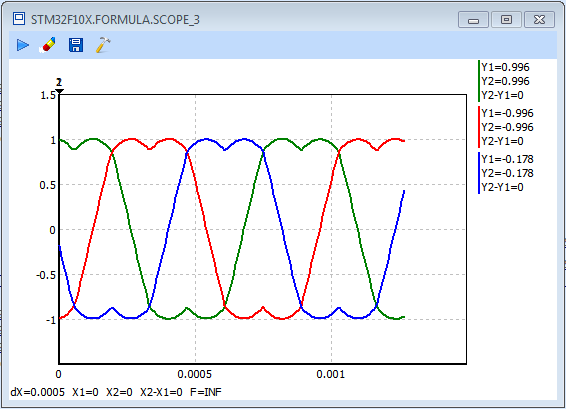
\includegraphics[width=0.8\linewidth]{8871_scope.png}}  \\
%\end{minipage}
\end{center}
\end{figure}
	Расходы ШИМ в блоке без перехода к декартовым координатам \cite{source}
\end{frame}


%\begin{frame}
%\frametitle{\smallфото установки}
%\begin{figure}
%\begin{center}
%\center{\includegraphics[width=1\linewidth]{ustanovka.jpg}}  \\
%\end{center}
%\end{figure}

%\end{frame}

\begin{frame}
\frametitle{\smallЛитература}
	\small{
\begin{thebibliography}{7}
	\bibitem{Gorev}Горев А.А. Переходные процессы синхронной машины. -- М.,Л., Гос. энергетическое изд., 1950. -- 551 c.
        \bibitem{Sokolovsky}Соколовский Г.Г. Электроприводы переменного тока с частотным регулированием: Учебник для студ. высш.учеб.заведений.
                -- М. «Академия», 2007 - 272 с.
%	\bibitem{Proshivka}Заливка прошивки в STM32 через USB \url{https://habr.com/post/403007/}
%	\bibitem{Zagruzchik}Программа-загрузчик \url{github.com/rogerclarkmelbourne/Arduino\_STM32}
	\bibitem{MexBios}Мехбиос \url{http://www.mechatronica-pro.com}
	\bibitem{source} Исходный код блока \url{https://github.com/trot-t/RemoteLabs}
%	\bibitem{ControlSUITE} \url{https://www.ti.com/tool/CONTROLSUITE}
		%описание на русском https://habr.com/post/403007/\\
%на английском %http://www.rogerclark.net/stm32f103-and-maple-maple-mini-with-arduino-1-5-x-ide/
%
%       Сама  программа загрузчик -- \\
%{\small https://github.com/rogerclarkmelbourne/Arduino\_STM32}

\end{thebibliography}
}
\end{frame}
\end{document}

